\chapter{Architecture and Implementation}
\label{ch:architecture-and-implementation}

\section{Architecture of the Software}

  \subsection{Adaptation Loop}

\section{Monitoring}

\section{Data Preprocessing and Analysis}

  \subsection{Alibaba Resource Analysis}
  \subsection{LSTM Architecture}
  \label{sec:lstm-architecture-and-implementation}

    The LSTM model was implemented with \nameref{sec:pytorch-evaluation-setup}, an open-source machine learning library for Python.
    \begin{figure}
      \centering
      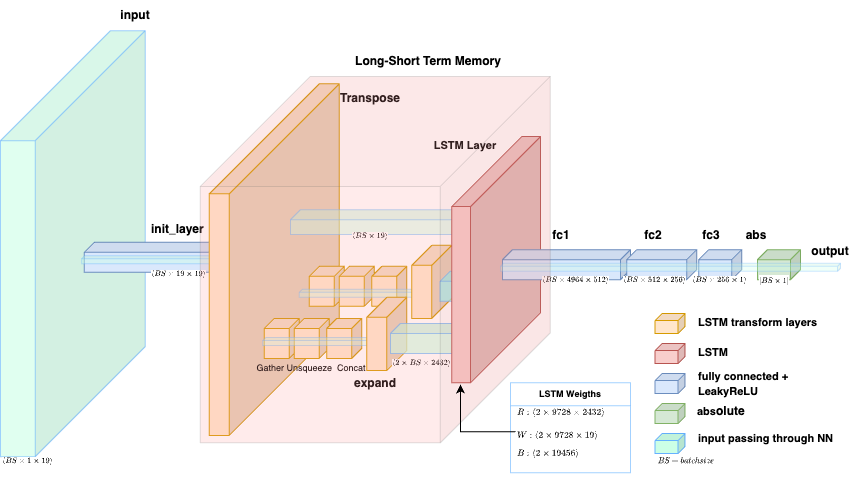
\includegraphics[scale=0.5]{figures/current_lstm_model.png}
      \caption{LSTM Model Architecture}
      \label{fig:lstm-model-architecture}
    \end{figure}
    As can be seen in figure \ref{fig:lstm-model-architecture} the input vector consisting of a pipeline task batch is forwarded to the \emph{initial layer}. This initial layer then creates an internal state and the initial hidden state

  % \lstinputlisting[
  %   language=Python, 
  %   caption=LSTM Architecture, 
  %   label=lst:pmse-python-class,
  %   captionpos=b,
  %   keywordstyle=\color{blue},
  %   frame=single,
  %   morekeywords={torch, nn, Module, Tensor, self},
  %   backgroundcolor=\color{gray!10!white},
  %   breaklines=true,
  %   numberstyle=\tiny\color{black},
  %   numbers=left,
  %   ]{code_samples/lstm_architecture.py}

  

\section{Adaptation}
  \subsection{Resource Prediction}
  % flow chart of resource prediction
  \subsection{DataFrame Scaler}
  \subsection{Penalty Mean Squared Error Loss Function}
  \label{sec:penalty-mse-loss-function-architecture-and-implementation}

    The \emph{Penalty Mean Squared Error (PMSE) loss function} is a custom loss function based on the commonly used \emph{Mean Squared Error (MSE) loss function} \cite{koksoyMultiresponseRobustDesign2006}:

    $$MSE = \frac{1}{N} \sum_{i = 1}^{N}\left(y_i - \hat{y}_i\right)^2$$

    \lstinputlisting[
      language=Python, 
      caption=Penalty Mean Squared Error Python Class, 
      label=lst:pmse-python-class,
      captionpos=b,
      keywordstyle=\color{blue},
      frame=single,
      morekeywords={torch, nn, Module, Tensor, self},
      backgroundcolor=\color{gray!10!white},
      ]{code_samples/pmse.py}


